\documentclass{beamer}
\usepackage[utf8]{inputenc}
\usepackage{hyperref}

\usepackage{utopia}

\usetheme{Madrid}
\usecolortheme{default}

%------------------------------------------------------------
\title[JURECA]
{JURECA}

\subtitle{First modular supercomputer worldwide}

\author[Claudio Scheer]
{Claudio~Scheer\inst{1}}

\institute[PUCRS]
{
  \inst{1}%
  Master's Degree in Computer Science\\
  Pontifical Catholic University of Rio Grande do Sul - PUCRS
}

\date[June 2020]
{Parallel Architectures, June 2020}
%------------------------------------------------------------


%------------------------------------------------------------
\AtBeginSection[]
{
  \begin{frame}
    \frametitle{Table of Contents}
    \tableofcontents[currentsection]
  \end{frame}
}
%------------------------------------------------------------


\begin{document}

\frame{\titlepage}

%---------------------------------------------------------
\begin{frame}
  \frametitle{Table of Contents}
  \tableofcontents
\end{frame}
%---------------------------------------------------------


%---------------------------------------------------------
\section{Curiosities}

\begin{frame}
  \frametitle{Organization}

  \begin{itemize}
    \item Forschungszentrum Jülich is a interdisciplinary research centre in Germany;
    \item Institute for Advanced Simulation (IAS);
    \item Jülich Supercomputing Centre (JSC);
          \begin{itemize}
            \item Supercomputing centre since 1987;
          \end{itemize}
  \end{itemize}
\end{frame}

\begin{frame}
  \frametitle{Managed supercomputers}
  \begin{itemize}
    \item JUSUF;
    \item JUWELS (position 31\footnote{November 2019 ranking.});
          \begin{itemize}
            \item Helped Google demonstrate the quantum supremacy~\href{https://www.fz-juelich.de/SharedDocs/Pressemitteilungen/UK/EN/2019/2019-10-23-quantum-Supremacy.html}{(source)};
                  \begin{itemize}
                    \item Quantum computer: 200 seconds;
                    \item Fastest supercomputer: 10.000 years;
                  \end{itemize}
          \end{itemize}
    \item JURECA (position 56\footnotemark[\value{footnote}]);
          \begin{itemize}
            \item The name is short for Jülich Research on Exascale Cluster Architectures;
          \end{itemize}
  \end{itemize}
\end{frame}

\begin{frame}
  \frametitle{JURECA}
  \begin{itemize}
    \item 2015-04: begins to operate the cluster;
    \item 2017-11: included a buster module;
    \item First modular supercomputer worldwide~\href{https://www.fz-juelich.de/SharedDocs/Pressemitteilungen/UK/EN/2017/2017-11-13-jureca-booster.html}{(source)};
  \end{itemize}
\end{frame}
%---------------------------------------------------------


%---------------------------------------------------------
\section{Architecture}

\begin{frame}
  \frametitle{JURECA Cluster}
  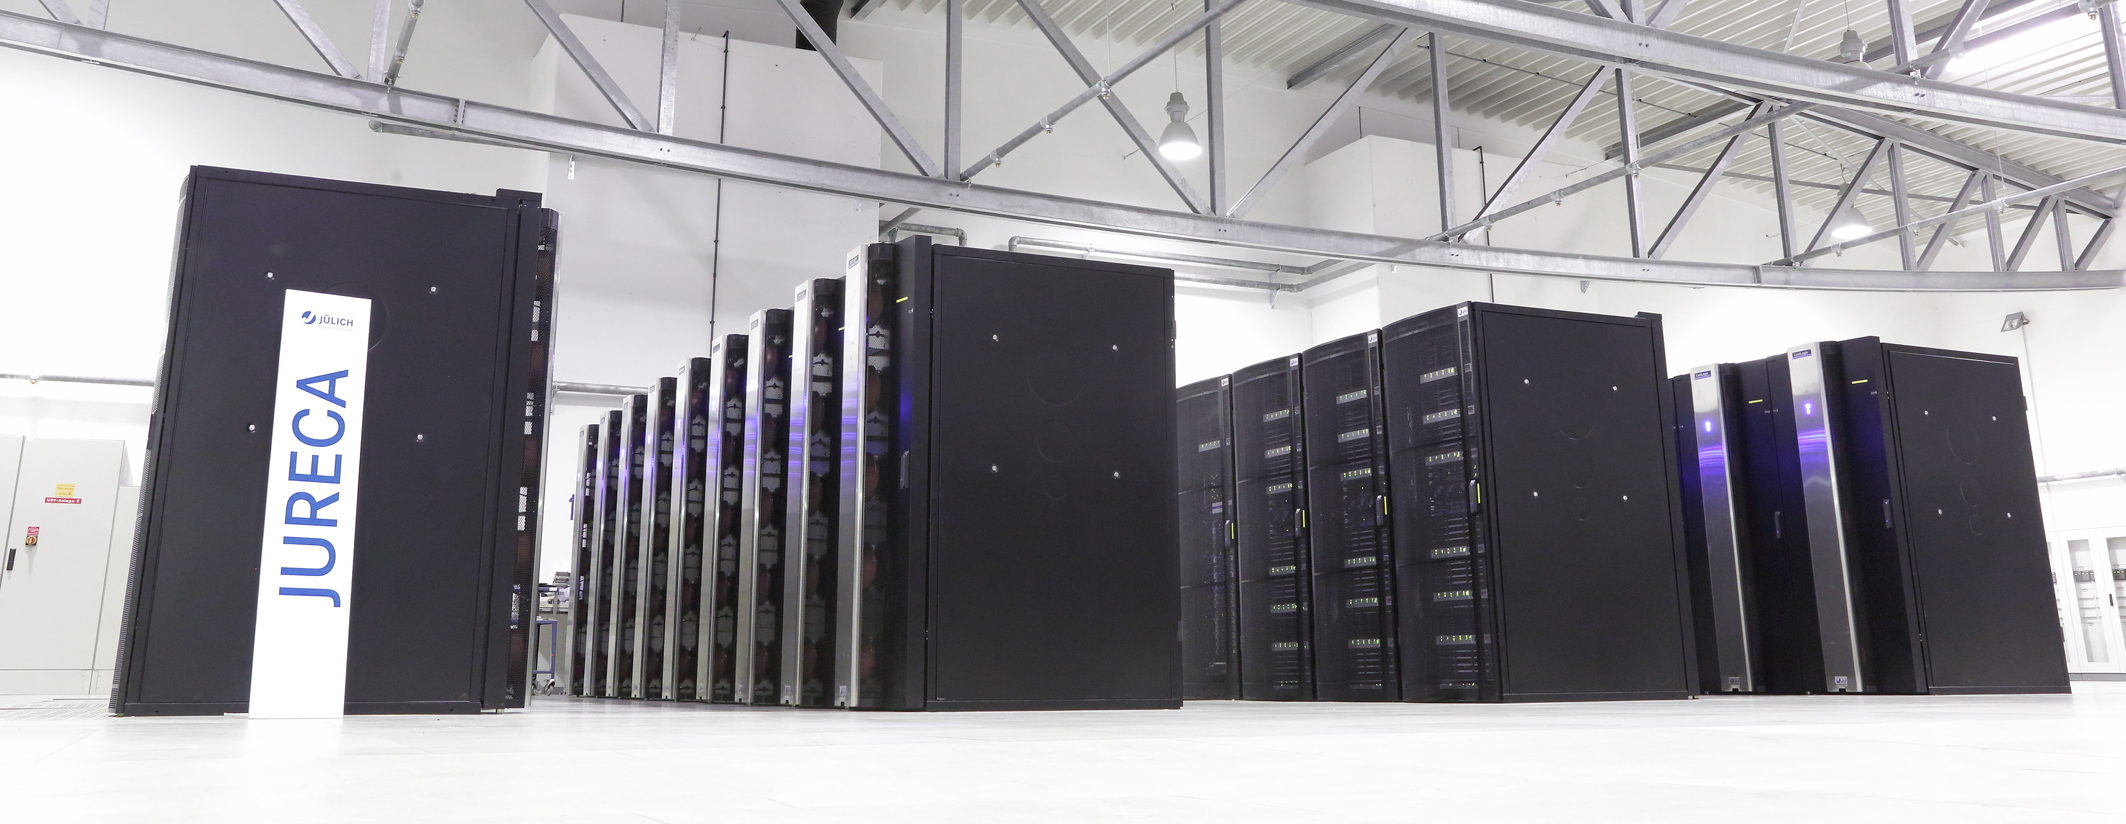
\includegraphics[width=\textwidth]{./images/jureca-cluster.jpeg}
\end{frame}

\begin{frame}
  \frametitle{JURECA Cluster}
  \begin{itemize}
    \item 1872 compute nodes\footnote{You can see the details \href{https://www.fz-juelich.de/ias/jsc/EN/Expertise/Supercomputers/JURECA/Configuration/Configuration_node.html}{here}.}
          \begin{itemize}
            \item 2 Intel Xeon E5-2680 v3 Haswell CPUs per node
                  \begin{itemize}
                    \item 2 x 12 cores, 2.5 GHz
                  \end{itemize}
            \item 75 compute nodes with 2 NVIDIA K80 GPUs
                  \begin{itemize}
                    \item 2 x 4992 CUDA cores
                    \item 2 x 24 GiB GDDR5 memory
                  \end{itemize}
            \item DDR4 memory (2133 MHz)
                  \begin{itemize}
                    \item 1605 compute nodes with 128 GiB memory
                    \item 128 compute nodes with 256 GiB memory
                    \item 64 compute nodes with 512 GiB memory
                  \end{itemize}
          \end{itemize}
  \end{itemize}
\end{frame}

\begin{frame}
  \frametitle{JURECA Cluster}
  \begin{itemize}
    \item 12 visualization nodes
          \begin{itemize}
            \item 2 Intel Xeon E5-2680 v3 Haswell CPUs per node
            \item 2 NVIDIA K40 GPUs per node
                  \begin{itemize}
                    \item 2 x 12 GiB GDDR5 memory
                  \end{itemize}
            \item 10 nodes with 512 GiB memory
            \item 2 nodes with 1024 GiB memory
          \end{itemize}
  \end{itemize}
\end{frame}

\begin{frame}
  \frametitle{Summary - JURECA Cluster}
  \begin{itemize}
    \item 1872 compute nodes
    \item 12 visualization nodes
    \item 45.216 CPU cores
    \item 1.8 (CPU) + 0.44 (GPU) Petaflop per second
    \item 100 GiB per second storage connection
  \end{itemize}
\end{frame}

\begin{frame}
  \frametitle{JURECA Buster}
  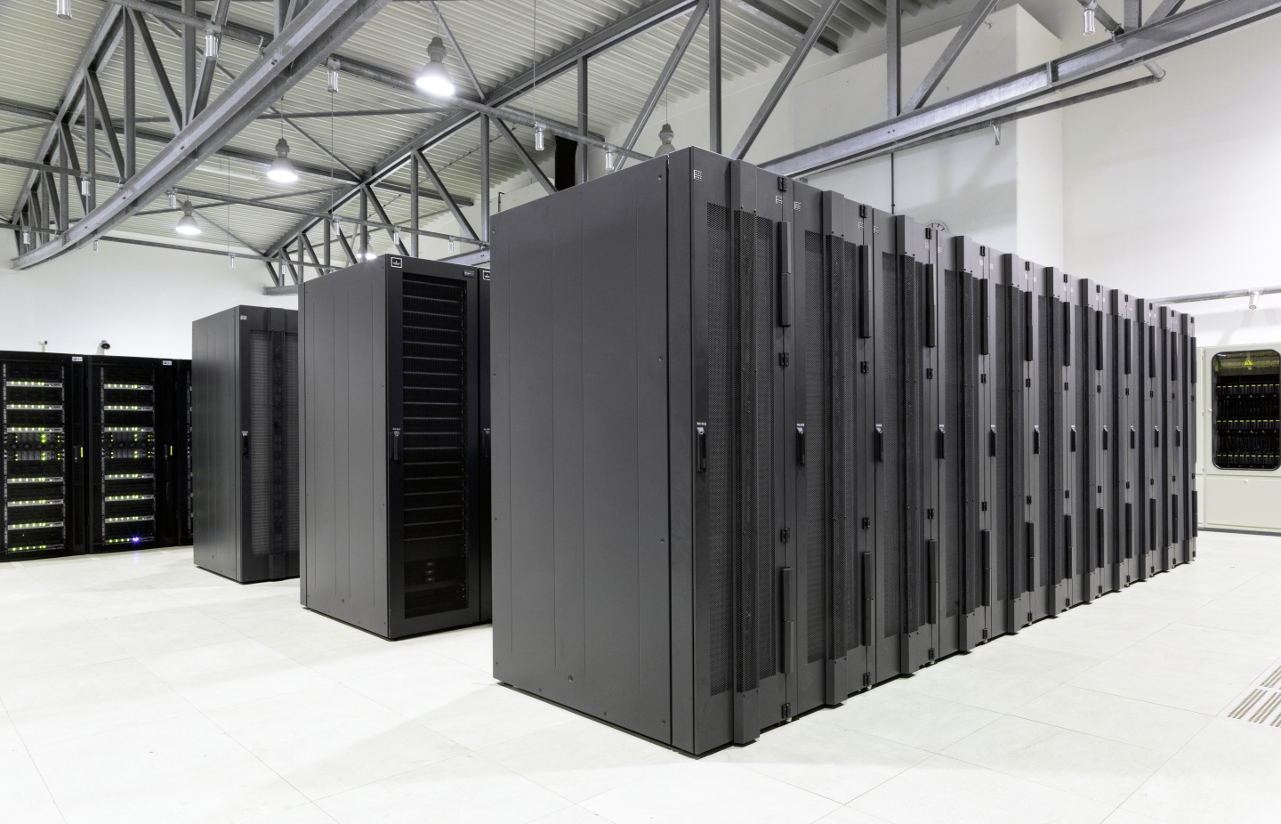
\includegraphics[width=\textwidth]{./images/jureca-buster.jpeg}
\end{frame}

\begin{frame}
  \frametitle{Summary - JURECA Buster}
  \begin{itemize}
    \item 1640 compute nodes\footnote{You can see the details \href{https://www.fz-juelich.de/ias/jsc/EN/Expertise/Supercomputers/JURECA/Configuration/Configuration_node.html}{here}.}
          \begin{itemize}
            \item 1 Intel Xeon Phi 7250-F Knights Landing CPUs per node
                  \begin{itemize}
                    \item 68 cores, 1.4 GHz
                    \item 96 GiB memory plus 16 GiB MCDRAM high-bandwidth memory
                  \end{itemize}
          \end{itemize}
    \item 111.520 CPU cores
    \item 5 Petaflop per second
    \item 100+ GiB per second storage connection
  \end{itemize}
\end{frame}

\begin{frame}
  \frametitle{Softwares}
  \begin{itemize}
    \item CentOS 7 Linux distribution
    \item Intel MPI and ParTec MPI
    \item OpenMP
    \item ...
  \end{itemize}
\end{frame}
%---------------------------------------------------------


%---------------------------------------------------------
\section{Classifications}

\begin{frame}
  \frametitle{Flynn}
  Based on the instruction stream and the data stream.

  \begin{itemize}
    \item SISD
    \item SIMD
    \item MISD
    \item \textbf{MIMD}
  \end{itemize}
\end{frame}

\begin{frame}
  \frametitle{Memory sharing}
  They use MPI to communicate between nodes.

  \begin{itemize}
    \item Multiprocessor
    \item \textbf{Multicomputer}
  \end{itemize}

  % https://youtu.be/LeBRG7dRZ08?t=4860
\end{frame}

\begin{frame}
  \frametitle{Type of memory access}
  \begin{itemize}
    \item UMA
    \item NUMA
    \item COMA
    \item \textbf{NORMA}
  \end{itemize}
\end{frame}

\begin{frame}
  \frametitle{Construction trends}
  \begin{itemize}
    \item PVP
    \item SMP
    \item MPP
    \item NOW
    \item \textbf{COW}
  \end{itemize}

  % https://youtu.be/dsFCeEW0qxU
\end{frame}

\begin{frame}
  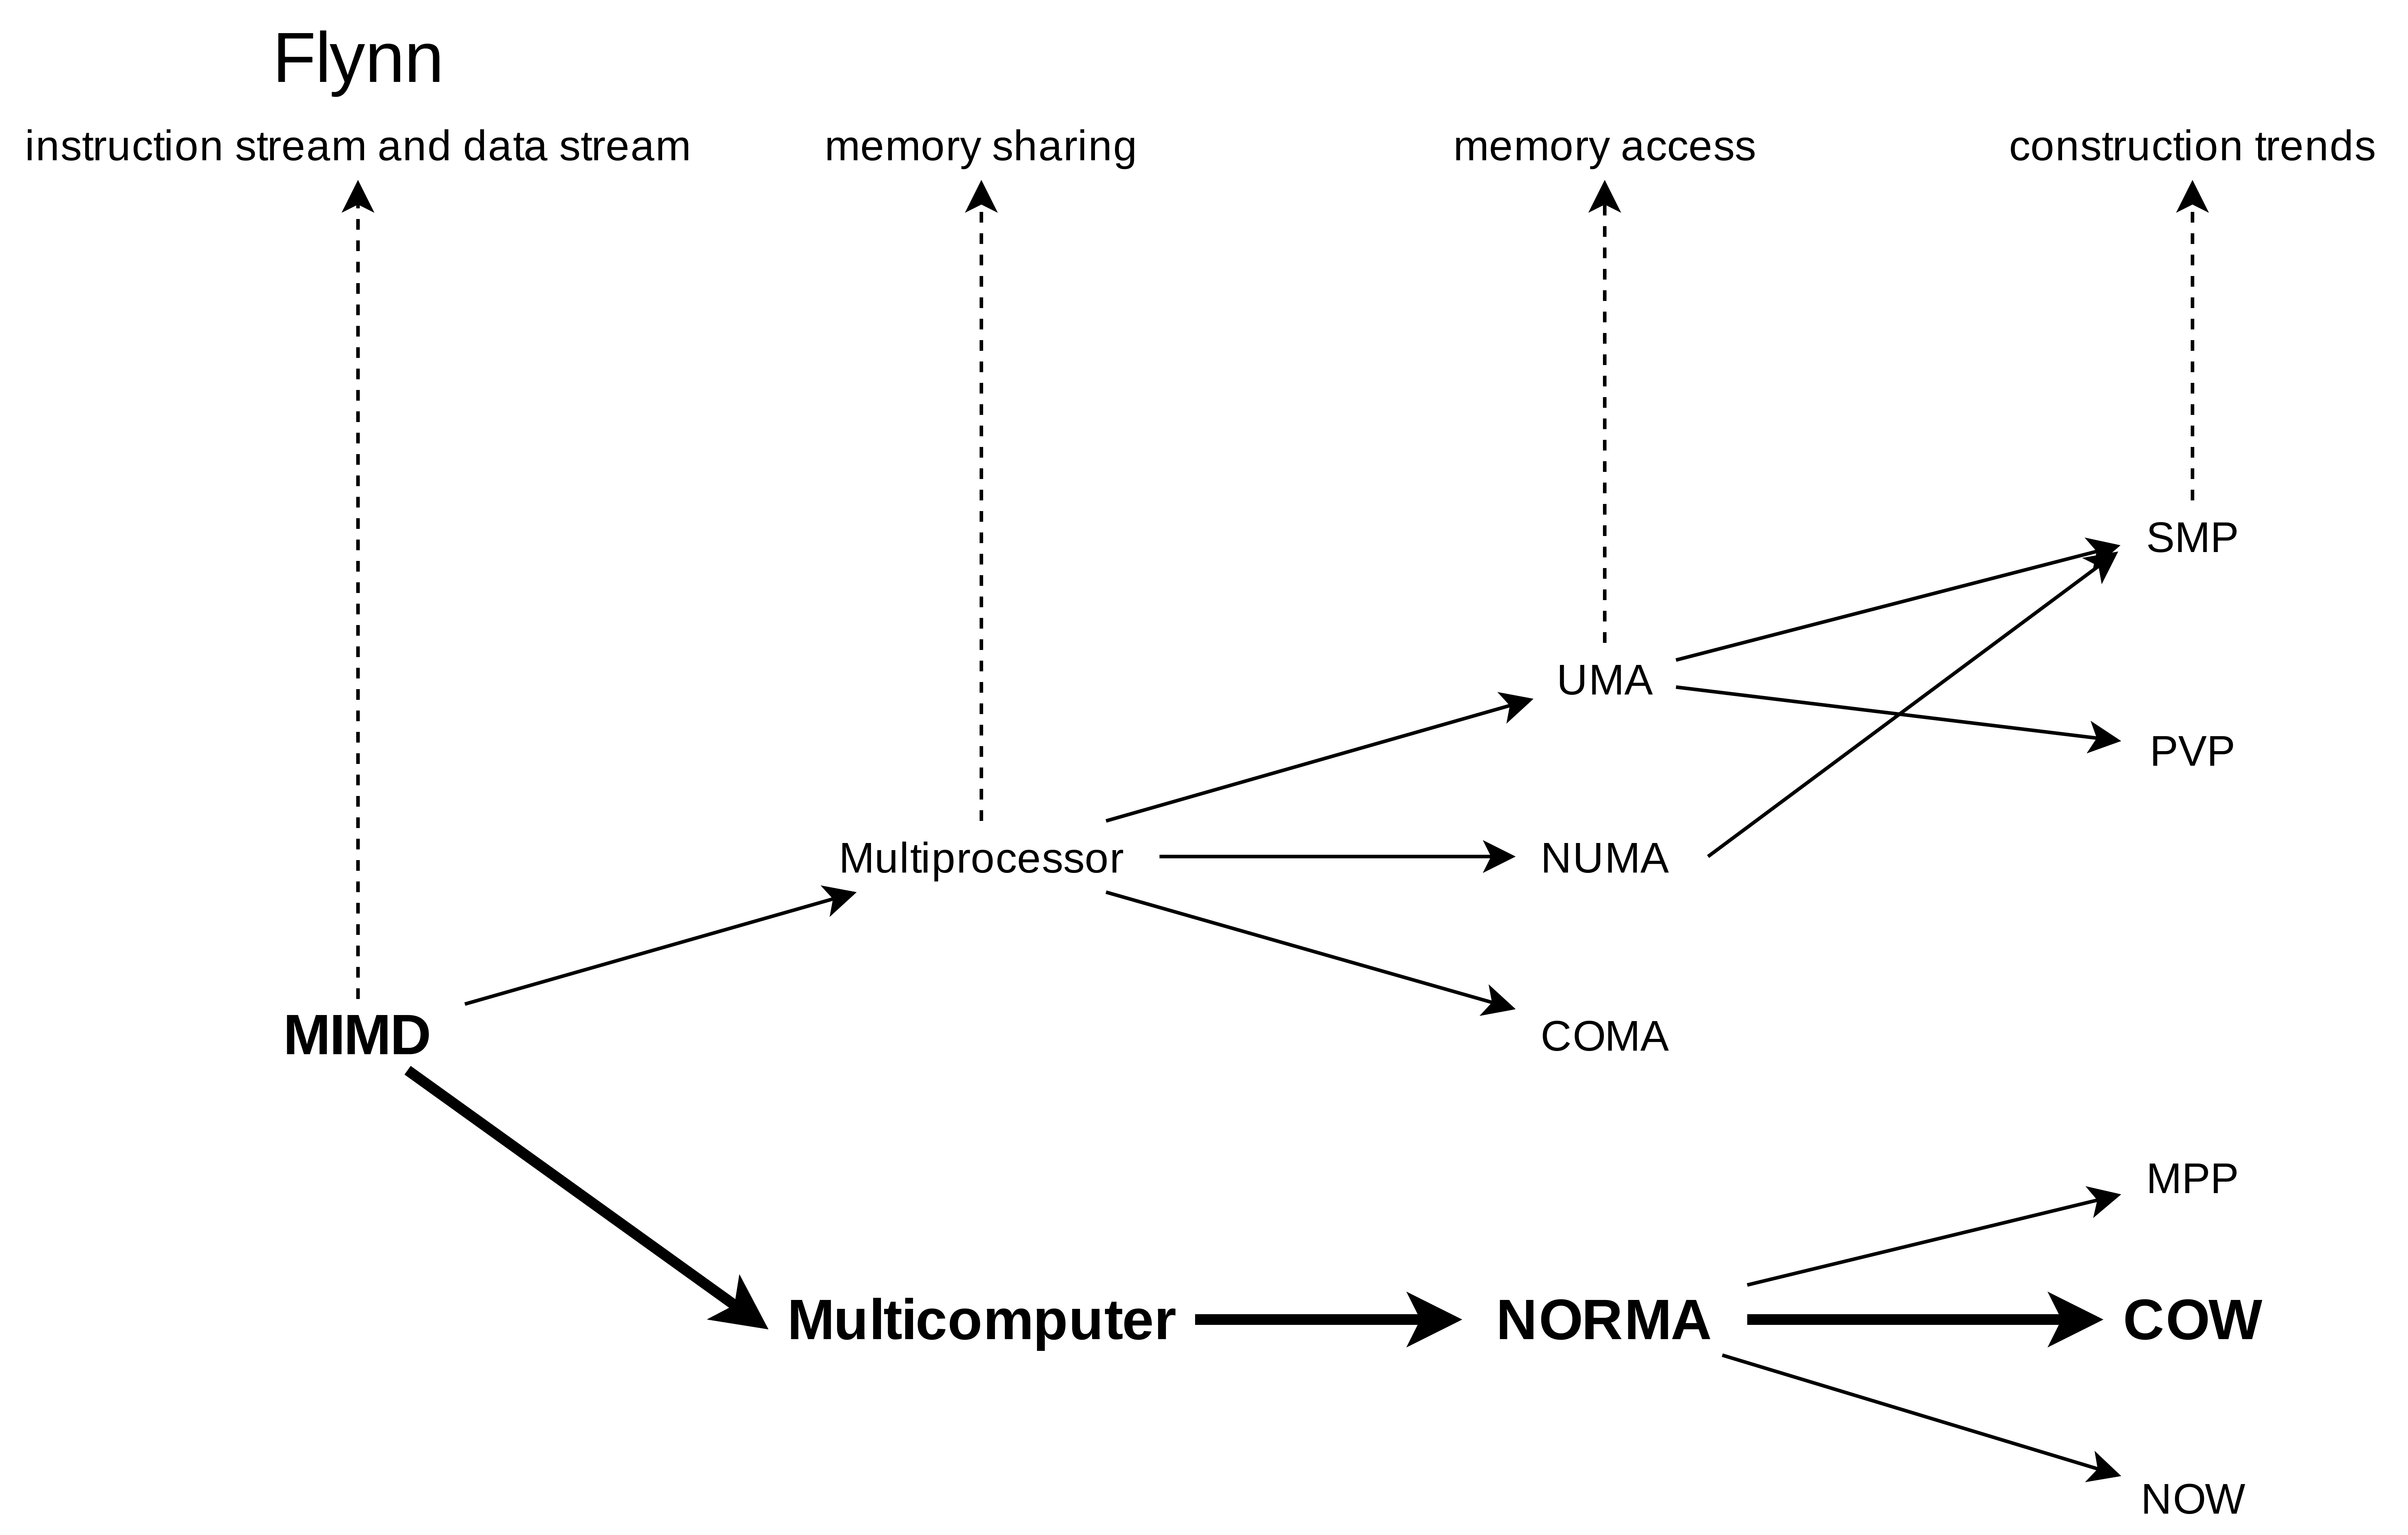
\includegraphics[width=\textwidth]{./images/classifications.png}
\end{frame}

\begin{frame}
  \frametitle{Flynn}
\end{frame}
%---------------------------------------------------------


%---------------------------------------------------------
\section{Other resources}

\begin{frame}
  \frametitle{Other resources}
  \begin{itemize}
    \item \href{https://www.youtube.com/watch?v=7h6mYU2HDTA}{Time lapse video of the installation}
    \item \href{https://www.fz-juelich.de/ias/jsc/EN/Home/home_node.html}{Jülich Supercomputing Centre}
  \end{itemize}
\end{frame}
%---------------------------------------------------------

\end{document}